\documentclass[UTF8,a4paper,zihao=-4,fontset=fandol]{ctexart}
\usepackage[left=24mm,right=24mm,top=22mm,bottom=22mm,headheight=15pt,headsep=6mm,footskip=10mm]{geometry}
\usepackage{amsmath,amssymb,amsthm,mathtools}
\usepackage{graphicx,booktabs,array}
\usepackage{caption,placeins}
\usepackage[numbers,sort&compress]{natbib}
\usepackage{fancyhdr}
\usepackage[hidelinks,unicode]{hyperref}
\usepackage{url}
\setmainfont[BoldFont=texgyretermes-bold.otf,ItalicFont=texgyretermes-italic.otf,BoldItalicFont=texgyretermes-bolditalic.otf]{texgyretermes-regular.otf}
\graphicspath{{figures/}}
\linespread{1.06}
\setlength{\parskip}{1pt}
\setlength{\textfloatsep}{12pt plus 2pt minus 2pt}
\setlength{\intextsep}{10pt plus 2pt minus 2pt}
\setlength{\floatsep}{10pt plus 2pt minus 2pt}
\renewcommand{\topfraction}{0.93}
\renewcommand{\bottomfraction}{0.80}
\renewcommand{\textfraction}{0.06}
\renewcommand{\floatpagefraction}{0.82}
\setcounter{topnumber}{3}
\setcounter{bottomnumber}{2}
\setcounter{totalnumber}{4}
\captionsetup{font=small,labelfont=bf,labelsep=quad,skip=5pt}
\ctexset{
  section={format=\large\bfseries,beforeskip=14pt,afterskip=7pt},
  subsection={format=\normalsize\bfseries,beforeskip=10pt,afterskip=5pt}
}
\pagestyle{fancy}
\fancyhf{}
\fancyhead[L]{\small 上海交通大学《概率论与数理统计》课程大作业}
\fancyhead[R]{}
\fancyfoot[C]{\thepage}
\renewcommand{\headrulewidth}{0.3pt}
\numberwithin{equation}{section}
\newtheorem{proposition}{命题}[section]
\renewcommand{\proofname}{证明}
\newcommand{\E}{\mathbb E}
\newcommand{\V}{\operatorname{Var}}
\newcommand{\SD}{\operatorname{SD}}
\newcommand{\Prob}{\mathbb P}
\newcommand{\ind}{\mathbf 1}
\newcommand{\CV}{\operatorname{CV}}
\newcommand{\given}{\,\middle|\,}
\newcommand{\BaseP}{0.098814}
\newcommand{\BaseMu}{16.914286}
\newcommand{\BaseConditionalVar}{54.213706}
\newcommand{\BaseMean}{1.671372}
\newcommand{\BaseVar}{30.833666}
\newcommand{\BaseWithin}{5.357086}
\newcommand{\BaseActivation}{25.476581}
\newcommand{\BaseZero}{0.904490}
\newcommand{\BaseTail}{0.338788}
\newcommand{\BaseOverallTail}{0.033477}

\hypersetup{
  pdftitle={随机卡组构筑中的组合可及性与收益稳定性研究},
  pdfauthor={Anonymous},
  pdfsubject={概率论与数理统计课程大作业},
  pdfkeywords={超几何分布，条件概率，全方差公式，蒙特卡洛模拟}
}
\title{\vspace{-1.4em}\zihao{3}\bfseries 随机卡组构筑中的组合可及性\\与收益稳定性研究\\[0.3em]
  \zihao{-3}——以《杀戮尖塔2》消耗机制为例}
\author{\normalsize 匿名作者\\[-0.1em]
  \small 上海交通大学}
\date{\small 2026年11月16日}
\begin{document}
\maketitle
\vspace{-1.2em}
\begin{abstract}
有限随机牌组中的协同收益，同时受关键组件可及性与成功条件下的手牌构成影响。
本文从《杀戮尖塔2》的消耗机制抽象出均匀排列模型，以容斥和次序统计量刻画组件联合可及性、
首次见齐时间及顺序约束，以同一次洗牌中的两阶段抽样构造条件超几何混合分布。
在24张基准牌组上，固定规模的普通攻击牌与非攻击牌替换使条件收益均值成为一次函数、
方差成为开口向下的二次函数，后者在普通非攻击牌数为9时达到整数最大值。
全方差分解表明，基准总体方差的82.63\%来自成功与失败两类条件均值的差异。
操作成本改变结论：直接增加6张普通非攻击牌，条件均值由16.91升至20.22，
总体均值却由1.67降至1.04。107组配置的精确计算与独立随机排列模拟表明，
可及性、条件收益和总体波动随卡组增删与替换呈现不同变化规律。
\end{abstract}
\noindent\textbf{关键词：}超几何分布；条件概率；首次见齐时间；全方差公式；蒙特卡洛模拟
\section{引言}
协同组件的随机出现，是有限资源系统中的一类组合可及性问题。
单个组件进入样本的概率，无法直接说明多个组件何时共同出现；
即使组件齐全，后续收益也会随剩余资源构成而波动。
例如，一副24张牌的牌组中，某张指定牌进入前10张的概率为$10/24$，
而两个指定能力组件与一个可替代消耗组件共同进入前10张，需要计算另一个联合事件。
区分单组件出现、联合可及性与条件回报，是评价此类系统的基础。

《杀戮尖塔2》是一款以随机牌组构筑为核心的卡牌游戏\cite{steam}。
其中，消耗一张牌可以同时触发抽牌与防御收益，批量消耗则把一次随机手牌的类别构成转化为数值回报。
本文选择这一机制作为有限无放回抽样的实例：把能力组件、消耗组件与普通牌划分类别，
以固定观察预算研究组件形成的机会，再研究同一排列中随后样本的收益。
模型中的“格挡”表示可累加的防御点数。

本文围绕三个相互衔接的问题展开：关键组件的联合可及性与首次见齐时间如何变化，
同洗牌条件依赖如何决定消耗收益分布，以及构筑操作如何分别改变启动机会、条件回报和总体波动。
组合计数给出精确概率，交换性给出均值与方差关于牌类数量的结构表达，
全期望与全方差则把条件收益连接到总体指标。
本文以概率统计的基本工具\cite{blitzstein}进行推导，并用随机排列模拟检验数值结果及估计精度。

\clearpage
\section{抽象卡组与随机实验}\label{sec:model}
\subsection{类别、参数与样本空间}
设六类牌的数量分别为$a,b,c,d,t,s$，总数
$N=a+b+c+d+t+s$。基准构成见表\ref{tab:deck}。
同类牌仍有不同实体编号，样本空间由$N!$个等概率排列组成。
前$n$张是均匀的$n$元不放回样本；$h$表示其后的收益抽样张数，
满足$0\le n\le N$、$0\le h\le N-n$。
基准取$(N,n,h)=(24,10,4)$。
基准卡组包含核心能力、消耗组件和普通牌。
取$n=10$作为前期组件观察窗口，$h=4$作为收益抽样窗口，
使一张保留的C与四张随机牌组成五张收益手牌。
后文将比较不同卡组规模与类别数量下的概率与收益。

\begin{table}[htbp]
\centering\small
\caption{基准抽象卡组及固定机制}\label{tab:deck}
\begin{tabular}{clrp{9.3cm}}
\toprule
类别 & 机制原型 & 数量 & 模型中的作用\\
\midrule
A & 黑暗之拥 & 1 & 生效后，每消耗一张牌产生一次抽牌触发\\
B & 无惧疼痛 & 1 & 生效后，每消耗一张牌增加3点格挡\\
C & 重振精神 & 2 & 消耗其他非攻击牌，每张提供5点格挡\\
D & 恶魔之焰 & 1 & 消耗其余手牌；作为静态可及性分析中的备选消耗组件\\
T & 普通攻击牌 & 9 & 不属于C的消耗对象\\
S & 普通非攻击牌 & 10 & 可由C消耗\\
\bottomrule
\end{tabular}
\end{table}

A、B、C、S为非攻击类，D、T为攻击类。
公开卡牌资料中的抽牌、额外格挡、非攻击牌批量消耗与手牌批量消耗描述，
分别对应表中的四个机制原型\cite{dark,pain,wind,fire}。
本文采用未升级卡牌的基础效果，将每张消耗获得的$5+3=8$点格挡作为模型参数。

\subsection{可及性、顺序事件与两阶段协议}
定义$F_n^C$为前$n$张中A、B、C各至少出现一张的事件，
$F_n^E$则把C条件替换为“C或D至少出现一张”。
定义$O_n^C$、$O_n^E$为相应前缀中存在一张触发牌，
其位置严格晚于第一张A和第一张B的事件。
因此$O_n^q\subseteq F_n^q$，$q\in\{C,E\}$。
前缀较早出现的触发牌，可以与后来另一张满足顺序的触发牌并存。

收益实验使用同一排列，并依次执行以下协议。
揭示前$n$张，令$I=\ind_{F_n^C}$。
当$I=1$时，假想各激活一张A、B，保留一张已揭示C，其余已揭示牌退出本次实验；
收益手牌由保留的C与排列位置$n+1,\ldots,n+h$的牌组成。
令$X$为这$h$张中可被C消耗的非攻击牌数；当$I=0$时约定$X=0$。
C自身不计入$X$。条件收益为$G=8X$，总体收益定义为
\begin{equation}\label{eq:payoff-definition}
Y=IG=8IX,\qquad
p=\Prob(I=1),\quad
\mu=\E(G\mid I=1),\quad
\sigma^2=\V(G\mid I=1).
\end{equation}
此处条件均值与方差要求$p>0$。基准中A、B已经位于前缀，
故收益阶段的非攻击牌恰为C或S。

收益协议以$F_n^C$为成功条件，$O_n^C$用于单独考察出现顺序。
收益阶段统计A产生的抽牌触发次数$R=X$，并计算C与B共同产生的格挡；
D用于可及性比较。整个实验针对固定预算下的随机排列与消耗收益，
能量、抽牌反馈和牌堆循环作为后续的动态问题。
推广到多副本A/B时，协议各激活一张，其余未揭示副本按非攻击牌处理。

\section{关键组件的可及性与首次见齐时间}\label{sec:access}
\subsection{联合抽取概率与关键牌复制}
令三个互不重叠的必需类别数量为$m_1=a,m_2=b,m_3=k$，
其中C类问题取$k=c$，E类问题取$k=c+d$。
记$F_n$为三类各至少出现一张的事件。
对“遗漏某一类”的事件应用容斥，得到
\begin{equation}\label{eq:inclusion}
\Prob(F_n)=\sum_{J\subseteq\{1,2,3\}}(-1)^{|J|}
\frac{\binom{N-\sum_{j\in J}m_j}{n}}{\binom Nn}.
\end{equation}
约定上参数为负或下参数越界的组合数为0。
该式统一覆盖不同副本数量；也可通过枚举三类在前缀中的正计数得到相同的组合概率。

当$a=b=1$时，可先强制A、B进入前缀，再从其余$N-2$张中排除不含触发牌的子集：
\begin{equation}\label{eq:singleton}
\Prob(F_n)=
\frac{\binom{N-2}{n-2}-\binom{N-2-k}{n-2}}{\binom Nn}.
\end{equation}
由此，基准前10张的两种可及性分别为
\begin{equation}\label{eq:baseline-access}
\Prob(F_{10}^C)=\frac{25}{253}\approx0.098814,\qquad
\Prob(F_{10}^E)=\frac{63}{506}\approx0.124506.
\end{equation}
E类还允许D充当消耗组件，因此$F_n^C\subseteq F_n^E$，对应的可及性更高。

\begin{figure}[htbp]
\centering
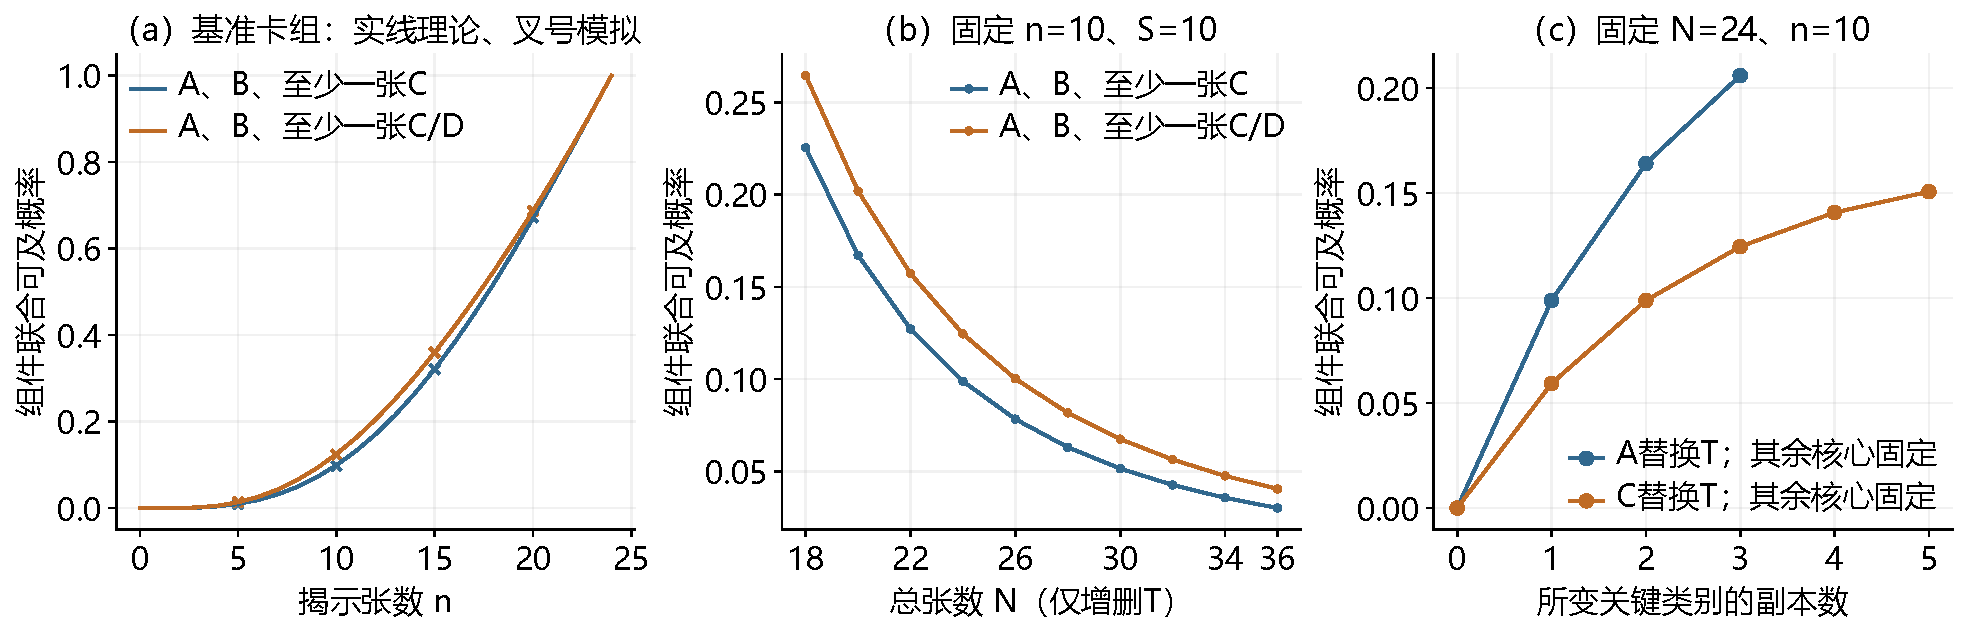
\includegraphics[width=\linewidth]{01_accessibility.pdf}
\caption{联合组件可及性。实线为精确理论值，左图叉号为每配置20万次排列模拟；
改变$N$通过增删T实现，复制关键牌通过固定$N$替换T实现。}\label{fig:access}
\end{figure}

图\ref{fig:access}中，可及性随观察预算$n$增加而上升；
固定核心数量而增加普通牌，会稀释固定前缀中的组件机会。
这两点也可通过同一随机排列中的插入或前缀延伸耦合证明。
对于$F_n^C$，固定$N,n,a=b=1$，并将一张非必需类别牌替换为C，
使C的数量由$c$增至$c+1$。由式\eqref{eq:singleton}与帕斯卡恒等式可得：
\begin{equation}\label{eq:marginal}
\Prob(F_n^C;c+1)-\Prob(F_n^C;c)
=\frac{\binom{N-3-c}{n-3}}{\binom Nn}.
\end{equation}
该增量随$c$非增，表明固定规模下复制C的边际收益递减。
若直接增加卡牌，总数$N$也随之变化；对$F_n^E$则以$c+d$为有效触发数，
例如把D替换为C时，$c+d$保持不变。

\subsection{首次见齐时间的分布与矩}
用$\tau_C,\tau_E$表示两类事件的首次见齐位置。
对任一类事件，令$\tau=\min\{n:F_n\text{成立}\}$。
当必需类别均存在时，$F_n$随$n$单调，因而
\begin{equation}\label{eq:time-pmf}
\Prob(\tau\le n)=\Prob(F_n),\qquad
\Prob(\tau=n)=\Prob(F_n)-\Prob(F_{n-1}).
\end{equation}
由逐样本恒等式$\tau=\sum_{n=0}^{N-1}\ind_{\{\tau>n\}}$及
$\tau^2=\sum_{n=0}^{N-1}(2n+1)\ind_{\{\tau>n\}}$，有
\begin{equation}\label{eq:tail-moments}
\E(\tau)=\sum_{n=0}^{N-1}\Prob(\tau>n),\qquad
\E(\tau^2)=\sum_{n=0}^{N-1}(2n+1)\Prob(\tau>n).
\end{equation}
再减去$\E(\tau)^2$即得方差。分位数统一取
$q_\alpha=\min\{n:\Prob(\tau\le n)\ge\alpha\}$。
基准精确结果见表\ref{tab:time}，其中
$\E(\tau_E)=205/12$、$\V(\tau_E)=25565/1008$，
$\E(\tau_C)=35/2$、$\V(\tau_C)=275/12$。

\begin{table}[htbp]
\centering\small
\caption{基准首次见齐时间的精确理论指标}\label{tab:time}
\begin{tabular}{lrrrrr}
\toprule
时间 & $\mathbb E(\tau)$ & $\operatorname{Var}(\tau)$ & $q_{0.5}$ & $q_{0.9}$ & $q_{0.95}$ \\
\midrule
$\tau_C$ & 17.500000 & 22.916667 & 18 & 23 & 24 \\
$\tau_E$ & 17.083333 & 25.362103 & 18 & 23 & 24 \\
\bottomrule
\end{tabular}

\end{table}

E类的均值较小，方差却较大，两类90\%分位数均为23张。
由于逐样本有$\tau_E\le\tau_C$，增加备选消耗组件缩短了平均见齐时间，
却使方差增大，体现出均值与离散程度的不同变化。
将容斥代入尾和，还可得到
\begin{equation}\label{eq:time-general-mean}
\E(\tau)=(N+1)
\sum_{\varnothing\ne J\subseteq\{1,2,3\}}
\frac{(-1)^{|J|+1}}{1+\sum_{j\in J}m_j}.
\end{equation}
这里使用恒等式
$\sum_{n=0}^{N-1}\binom{N-m}{n}/\binom Nn=(N+1)/(m+1)$；
右侧也等于$m$个指定位置的最小次序统计量期望。
固定关键类别数量时，首次见齐时间的期望与$N+1$成正比。

\subsection{有限前缀中的顺序约束}
仍取$a=b=1$。令$j$为A、B位置中较后者，则
$\Prob(\max(\operatorname{pos}A,\operatorname{pos}B)=j)
={2(j-1)}/{[N(N-1)]}$。
给定这两位置，$k$张触发牌均匀占据其余$N-2$个位置。
前缀中可满足顺序的位置为$j+1,\ldots,n$，共有$n-j$个。
用补集排除这些位置没有触发牌的情况，得
\begin{equation}\label{eq:order}
\Prob(O_n)=\sum_{j=2}^{n-1}\frac{2(j-1)}{N(N-1)}
\left[1-\frac{\binom{N-2-(n-j)}{k}}{\binom{N-2}{k}}\right].
\end{equation}
抽完整副牌时，$k+2$张关键牌的最后一张属于触发类的概率为
$\Prob(O_N)=k/(k+2)$。对有限前缀则用式\eqref{eq:order}计入触发牌实际出现数量。

\begin{figure}[htbp]
\centering
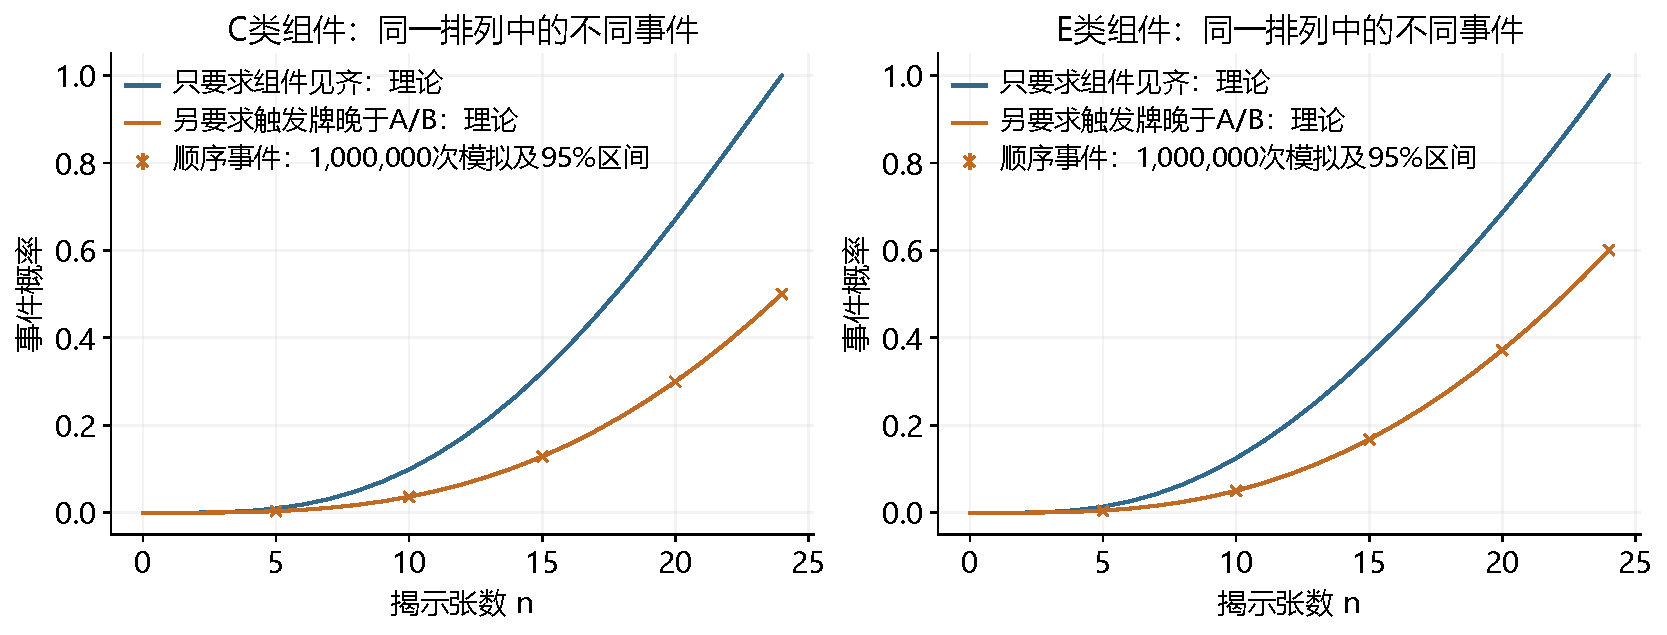
\includegraphics[width=\linewidth]{03_order_constraint.pdf}
\caption{组件见齐与顺序事件的精确概率；叉号及95\% Wilson区间来自独立100万次排列模拟。}\label{fig:order}
\end{figure}

基准$n=10$时，$\Prob(O_{10}^C)=5/138\approx0.036232$，
$\Prob(O_{10}^E)=1/20=0.05$，分别为相应无序概率的36.67\%和40.16\%。
图\ref{fig:order}显示：即使抽完整副牌，无序事件概率达到1，
特定顺序事件的概率仍为$1/2$或$3/5$。
两种曲线的差距直观体现了抽牌次序对组件协同的影响。

\FloatBarrier
\section{同洗牌条件消耗收益的分布}\label{sec:conditional}
\subsection{由设置阶段计数构造联合概率}
两阶段样本来自同一排列。第一阶段抽走的类别数量，决定第二阶段的剩余组成，
所以应先给定设置阶段计数，再对条件分布求混合。
在基准中，成功时A、B均已揭示。
设前10张的C、S数量分别为$c_1,s_1$，其余为D或T，共有10张可选。
这些计数与$I=1$同时发生的无条件概率为
\begin{equation}\label{eq:setup-counts}
q(c_1,s_1)=
\frac{\binom2{c_1}\binom{10}{s_1}\binom{10}{8-c_1-s_1}}{\binom{24}{10}},
\qquad c_1\in\{1,2\},\quad 0\le s_1\le10.
\end{equation}
计数式中的组合数自动排除越界情况，$q$在全部设置计数上的和为$p$。
剩余$L=N-n=14$张中，可被C消耗的牌数为
$M(c_1,s_1)=(2-c_1)+(10-s_1)=12-c_1-s_1$。
给定计数后，未揭示部分仍是均匀排列，故
\begin{equation}\label{eq:hypergeometric}
\Prob(X=x\mid c_1,s_1,I=1)=
\frac{\binom{M(c_1,s_1)}x\binom{14-M(c_1,s_1)}{4-x}}{\binom{14}4},
\qquad x=0,\ldots,4.
\end{equation}
对互斥的设置阶段计数求和，得到联合概率质量
\begin{equation}\label{eq:joint}
J_x:=\Prob(X=x,I=1)=
\sum_{c_1=1}^2\sum_{s_1=0}^{10}q(c_1,s_1)
\frac{\binom{12-c_1-s_1}x\binom{2+c_1+s_1}{4-x}}{\binom{14}4}.
\end{equation}
每个超几何分布均归一，因此
$\sum_xJ_x=\sum_{c_1,s_1}q(c_1,s_1)=p$；
成功条件下的PMF为$J_x/p$，其权重为$q(c_1,s_1)/p$。

也可以先枚举收益位置$n+1,\ldots,n+h$的类别计数，
再从剩余实体中计算设置阶段的可及性。
两种条件化次序都得到$J_x$；研究中以精确有理数和小牌组全排列完成交叉验证。

\subsection{条件矩、尾概率与总体零收益}
基准条件PMF依次为
\begin{equation}\label{eq:conditional-pmf}
\bigl(\Prob(X=x\mid I=1)\bigr)_{x=0}^4
=\left(\frac{54}{1615},\frac{128}{595},\frac{933}{2261},
        \frac{636}{2261},\frac{130}{2261}\right).
\end{equation}
对式\eqref{eq:conditional-pmf}按$x$及$x^2$加权，
再将消耗数均值乘8、方差乘64，可得
\begin{equation}\label{eq:conditional-moments}
\begin{aligned}
\E(X\mid I=1)&=\frac{74}{35},\qquad
\V(X\mid I=1)=\frac{19716}{23275},\\
\mu&=\frac{592}{35}\approx\BaseMu,\qquad
\sigma^2=\frac{1261824}{23275}\approx\BaseConditionalVar.
\end{aligned}
\end{equation}
条件标准差约为7.3630，且
$\Prob(G\ge24\mid I=1)=766/2261\approx\BaseTail$。
对应的总体阈值概率为
$\Prob(Y\ge24)=p\Prob(G\ge24\mid I=1)\approx\BaseOverallTail$。
该式直接由联合事件$\{Y\ge24\}=\{I=1,G\ge24\}$得到。

\begin{figure}[htbp]
\centering
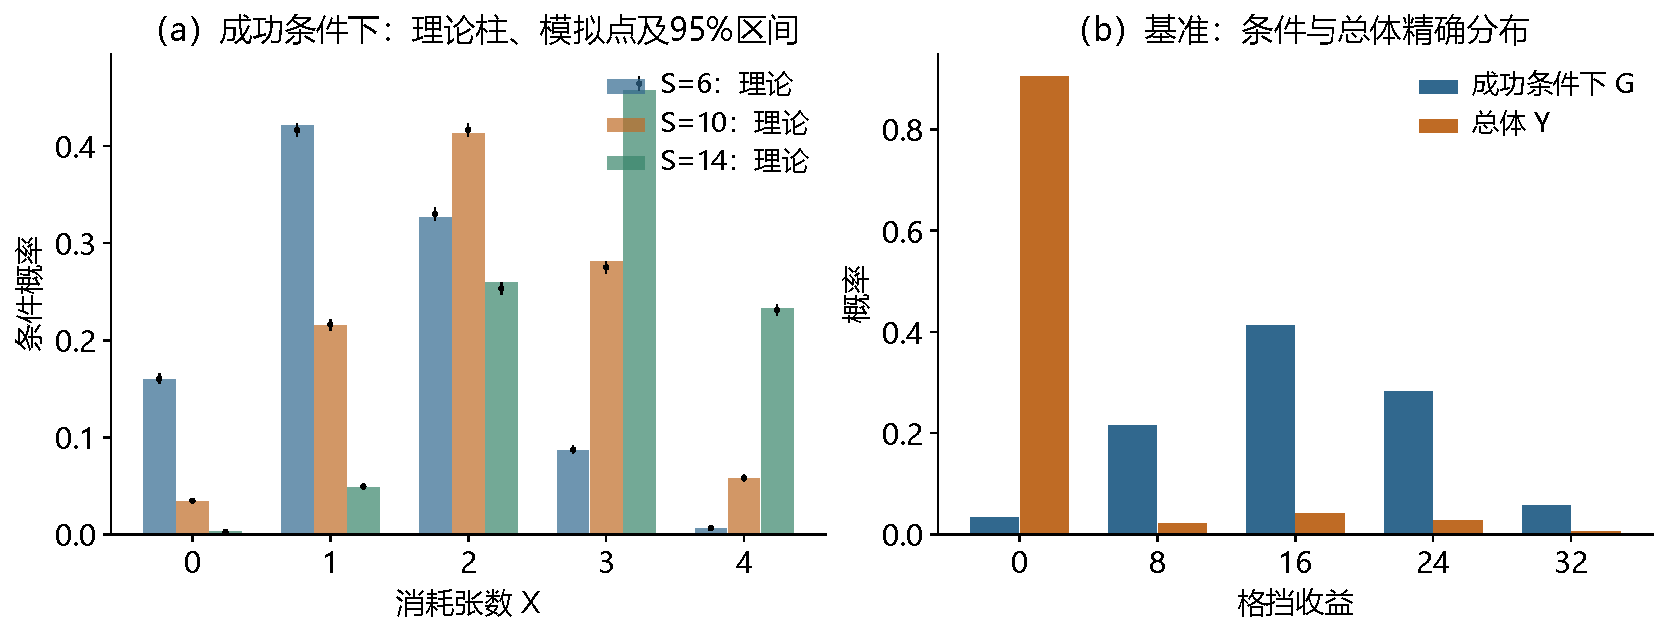
\includegraphics[width=\linewidth]{04_payoff_distributions.pdf}
\caption{条件消耗数量与收益分布。左图柱为精确理论值，点与区间来自每配置20万次模拟；
右图比较基准条件收益与总体收益的精确PMF。}\label{fig:distribution}
\end{figure}

图\ref{fig:distribution}右图的总体零收益概率为
\begin{equation}\label{eq:zero}
\Prob(Y=0)=1-p+J_0=\frac{73914}{81719}\approx\BaseZero.
\end{equation}
它同时包含组件未齐与组件齐全后$X=0$两种情况。
因此，基准总体90\%分位数为0，而条件90\%分位数为24。
更一般地，若$p\le0.1$，则$\Prob(Y=0)\ge1-p\ge0.9$，
非负总体收益的90\%分位数必为0。
对于这种零值集中的分布，阈值概率和条件分位数能补充总体分位数的区分能力。

\subsection{条件混合与独立重抽的区别}
若预先确定并移除一张A、B、C，再从剩余21张中重新均匀抽4张，
可消耗牌数为11，所定义的另一实验服从
$\operatorname{Hypergeom}(21,11,4)$，格挡均值为$352/21\approx16.761905$。
它与式\eqref{eq:conditional-moments}的差别，来自对前10张随机计数的不同处理。
独立重抽模型若沿用原协议的$p$，总体均值为1.656315；
同洗牌模型则为1.671372。两种抽样方式产生不同的条件分布。

条件混合的方差也有可解释的两层结构。
令$W=(c_1,s_1)$，$\theta=M(W)/L$。
在$L>1$时，超几何方差与全方差公式给出
\begin{equation}\label{eq:mixture-variance}
\V(X\mid I=1)=
h\frac{L-h}{L-1}\E\!\left[\theta(1-\theta)\mid I=1\right]
+h^2\V(\theta\mid I=1).
\end{equation}
式\eqref{eq:joint}的混合分布同时反映两层波动：
给定剩余组成后的无放回抽样波动，以及剩余组成本身的随机性。

\FloatBarrier
\section{构筑参数与收益稳定性}\label{sec:construction}
\subsection{交换性决定一次均值与二次方差}
固定$N=24$、$a=b=d=1$、$c=2$、$n=10$、$h=4$，
令普通非攻击牌数为$s$，普通攻击牌数为$t=19-s$，$0\le s\le19$。
必需组件数量保持不变，故$p=25/253$，而收益阶段可消耗牌的数量随$s$变化。

\begin{proposition}\label{prop:polynomial}
在上述固定规模替换下，条件收益均值与方差分别为
\begin{align}
\mu(s)&=\frac{64}{35}+\frac{264}{175}s,\label{eq:linear-mean}\\
\sigma^2(s)&=\frac{13824}{1225}
+\frac{1064832}{116375}s-\frac{282624}{581875}s^2.\label{eq:quadratic-variance}
\end{align}
条件方差在合法整数$s=9$时最大。
\end{proposition}

\begin{proof}
把A、B与两张C之外的20张实体牌暂视作普通实体。
启动事件$I=1$不区分这些实体的D、T、S标签。
记$Z$为收益阶段C的数量，$H_i$为第$i$张普通实体牌处于收益阶段的指示变量。
在其中固定选$s$张标记为S后，有
$X_s=Z+\sum_{i=1}^sH_i$。
成功时至少一张C已在前缀，故$Z\in\{0,1\}$。
下述期望均以$I=1$为条件。交换性保证
\[
z:=\E Z,\quad \alpha:=\E H_i,\quad
\beta:=\E(H_iH_j)\ (i\ne j),\quad
\gamma:=\E(ZH_i)
\]
与实体标签无关。
令$\phi(v,k)$表示总数为$v$、A/B各一张、C有$k$张的牌组，
前10张满足三类组件要求的概率；它由式\eqref{eq:singleton}给出。
一张指定实体进入收益阶段的概率为$4/24$，
两张指定实体共同进入的概率为$4\cdot3/(24\cdot23)$。
先指定收益实体，再在剩余牌中计算前缀事件，得到
\begin{equation}\label{eq:tagged-moments}
\begin{aligned}
z&=\frac{2(4/24)\phi(23,1)}p=\frac8{35},&
\alpha&=\frac{(4/24)\phi(23,2)}p=\frac{33}{175},\\
\beta&=\frac{[12/(24\cdot23)]\phi(22,2)}p=\frac{93}{3325},&
\gamma&=\frac{2[12/(24\cdot23)]\phi(22,1)}p=\frac6{175}.
\end{aligned}
\end{equation}
于是
\begin{equation}\label{eq:indicator-second}
\E X_s=z+s\alpha,\qquad
\E X_s^2=z+s\alpha+s(s-1)\beta+2s\gamma.
\end{equation}
将它们代入$\mu=8\E X_s$、
$\sigma^2=64[\E X_s^2-(\E X_s)^2]$，即得式
\eqref{eq:linear-mean}、\eqref{eq:quadratic-variance}。
方差二次项为$64(\beta-\alpha^2)<0$，
其连续顶点为$s_*=13865/1472\approx9.419158$。
最近的合法整数为9，故整数最大值在$s=9$取得。
\end{proof}

由上述矩表达式可见，条件均值由一阶矩确定，方差进一步取决于二阶矩及协方差项。
随着$s$增加，可消耗数量的均值上升；中等比例下两种牌类混合最明显，
接近两端时可消耗性更易确定，条件方差因而先升后降。
式\eqref{eq:tagged-moments}刻画了启动条件引起的牌组组成偏移。

\begin{figure}[htbp]
\centering
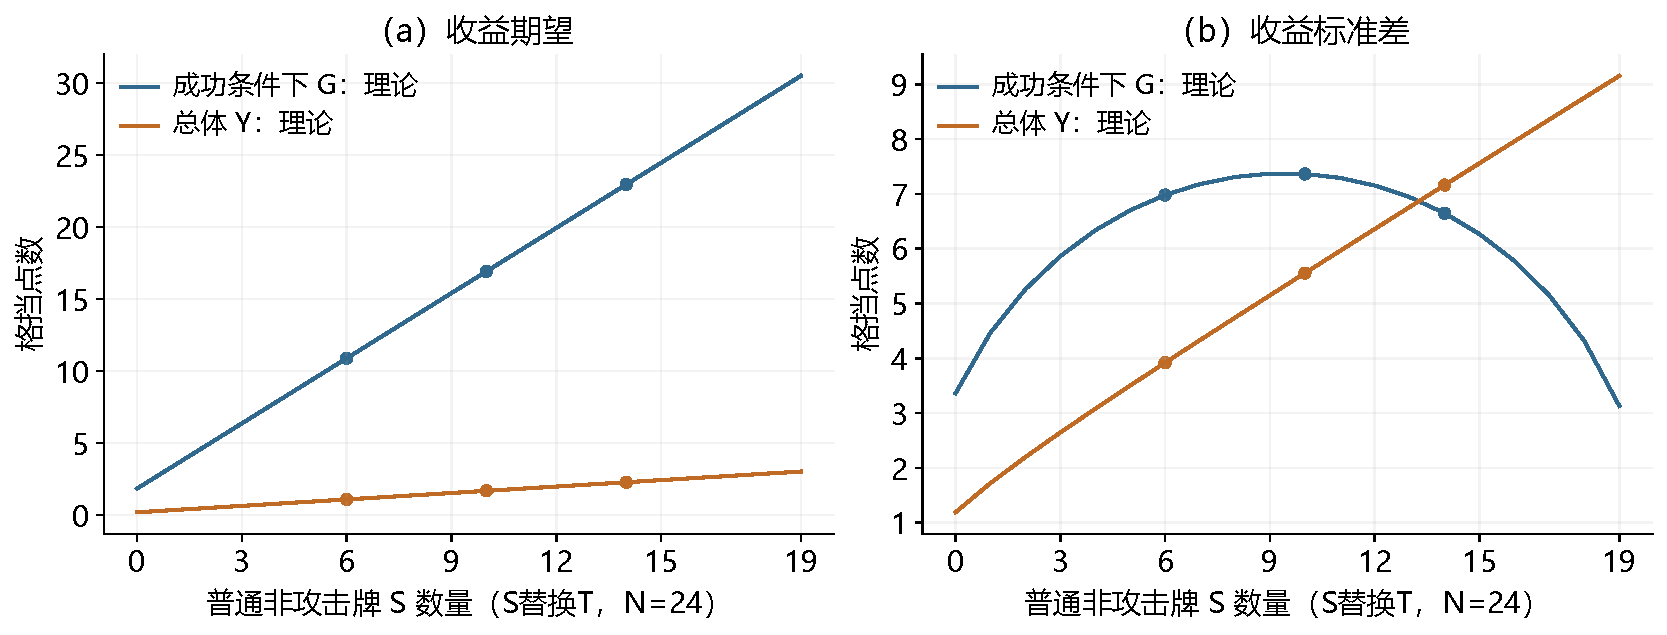
\includegraphics[width=\linewidth]{05_mean_and_sd.pdf}
\caption{固定$N$的S/T替换下，条件与总体收益的精确期望和标准差。
标记点对应$s=6,10,14$；右图显示方差指标与均值指标具有不同变化规律。}\label{fig:mean-sd}
\end{figure}

\begin{table}[htbp]
\centering\small
\caption{固定规模替换的代表性精确结果，三组均有$p=25/253$}\label{tab:baseline}
\begin{tabular}{rrrrrr}
\toprule
$s$ & $t$ & $\mu$ & $\sigma$ & $\mathbb E(Y)$ & $\operatorname{SD}(Y)$ \\
\midrule
6 & 13 & 10.8800 & 6.9785 & 1.0751 & 3.9183 \\
10 & 9 & 16.9143 & 7.3630 & 1.6714 & 5.5528 \\
14 & 5 & 22.9486 & 6.6472 & 2.2676 & 7.1598 \\
\bottomrule
\end{tabular}

\end{table}

图\ref{fig:mean-sd}和表\ref{tab:baseline}显示，条件标准差从$s=10$到14下降，
总体标准差却继续上升。不同层次的收益变量，具有不同的方差变化规律。
此外，在同一个实体排列中把一张T改标为S，$I$不变而$X$逐样本不减，
因此条件收益和总体收益均关于$s$一阶随机占优。
因此均值和正阈值尾概率随$s$非减，方差则遵循式\eqref{eq:quadratic-variance}的二次关系。

\subsection{全期望、全方差与零值混合}
在$I=0$时$Y=0$，在$I=1$时$Y=G$。
因此$\E(Y\mid I)=I\mu$、$\V(Y\mid I)=I\sigma^2$。
依次对$I$取期望与方差，得到
\begin{equation}\label{eq:total-moments}
\E(Y)=p\mu,\qquad
\V(Y)=
\underbrace{p\sigma^2}_{\text{成功后的条件波动}}
+\underbrace{p(1-p)\mu^2}_{\text{成功/失败条件均值差异}}.
\end{equation}
基准结果为
\begin{equation}\label{eq:total-values}
\E(Y)=\frac{2960}{1771}\approx\BaseMean,\qquad
\V(Y)\approx\BaseWithin+\BaseActivation=\BaseVar.
\end{equation}
两个方差贡献分别占17.3741\%与82.6259\%。
其中第二项体现成功与失败两类条件均值之间的差异。

\begin{figure}[htbp]
\centering
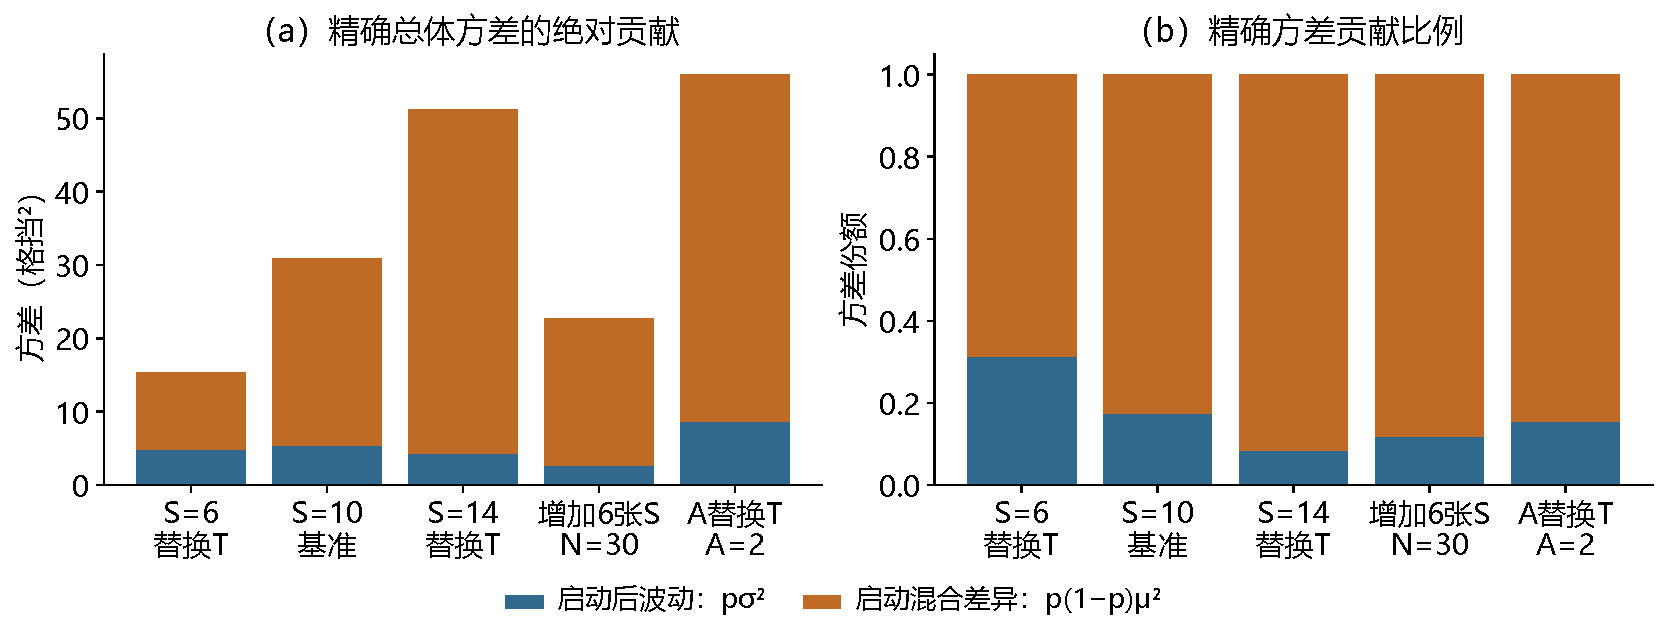
\includegraphics[width=\linewidth]{06_variance_decomposition.pdf}
\caption{不同操作下总体方差的精确分解。左图为绝对贡献，右图为份额；
基准中成功/失败条件均值差异占82.63\%。}\label{fig:variance}
\end{figure}

图\ref{fig:variance}显示，总体方差由条件波动和成功概率共同决定。
固定$p$时，均值$\mu$上升还会放大$p(1-p)\mu^2$，
从而解释图\ref{fig:mean-sd}中条件与总体标准差的不同走向。
当$\mu>0$时，记$\CV(U)=\SD(U)/\E(U)$，由式\eqref{eq:total-moments}还有
\begin{equation}\label{eq:cv}
\CV(Y)^2=\frac{\CV(G\mid I=1)^2+1-p}{p}.
\end{equation}
较小的$p$本身就会提高相对波动。
因此总体标准差、零收益概率与总体均值应联合解读。

\subsection{增删与替换操作的不同权衡}
表\ref{tab:operations}均以基准为参照，固定$n=10,h=4$。
增加或删除牌张改变$N$；替换保持$N$不变。
多副本A按第\ref{sec:model}节的协议激活一张，其余未揭示副本仍可被C消耗。

\begin{table}[htbp]
\centering\small
\caption{明确操作成本后的代表性构筑指标，均为精确理论值}\label{tab:operations}
\setlength{\tabcolsep}{5pt}
\begin{tabular}{lrrrrrr}
\toprule
相对基准操作 & $N$ & $p$ & $\mu$ & $\mathbb E(Y)$ & $\operatorname{SD}(Y)$ & $\mathrm{CV}(Y)$ \\
\midrule
基准 & 24 & 0.0988 & 16.9143 & 1.6714 & 5.5528 & 3.3223 \\
删除6张S & 18 & 0.2255 & 11.1304 & 2.5098 & 5.6406 & 2.2474 \\
增加6张S & 30 & 0.0515 & 20.2160 & 1.0401 & 4.7599 & 4.5763 \\
以A替换1张T & 24 & 0.1640 & 18.5640 & 3.0451 & 7.4803 & 2.4565 \\
以C替换1张T & 24 & 0.1245 & 18.5435 & 2.3088 & 6.6399 & 2.8760 \\
以C替换1张S & 24 & 0.1245 & 17.0483 & 2.1226 & 6.1989 & 2.9204 \\
\bottomrule
\end{tabular}

\end{table}

直接增加6张S，条件均值从16.9143提高到20.2160，
但启动概率从0.0988降到0.0515，总体均值从1.6714降到1.0401。
与固定$N$的S/T替换相比，这一操作额外引入了组件稀释。
图\ref{fig:tradeoff}展示了条件收益与组件可及性的权衡：
在所研究的S增删序列中，增加S提高条件回报，却降低固定预算内的组件齐全概率。

\begin{figure}[htbp]
\centering
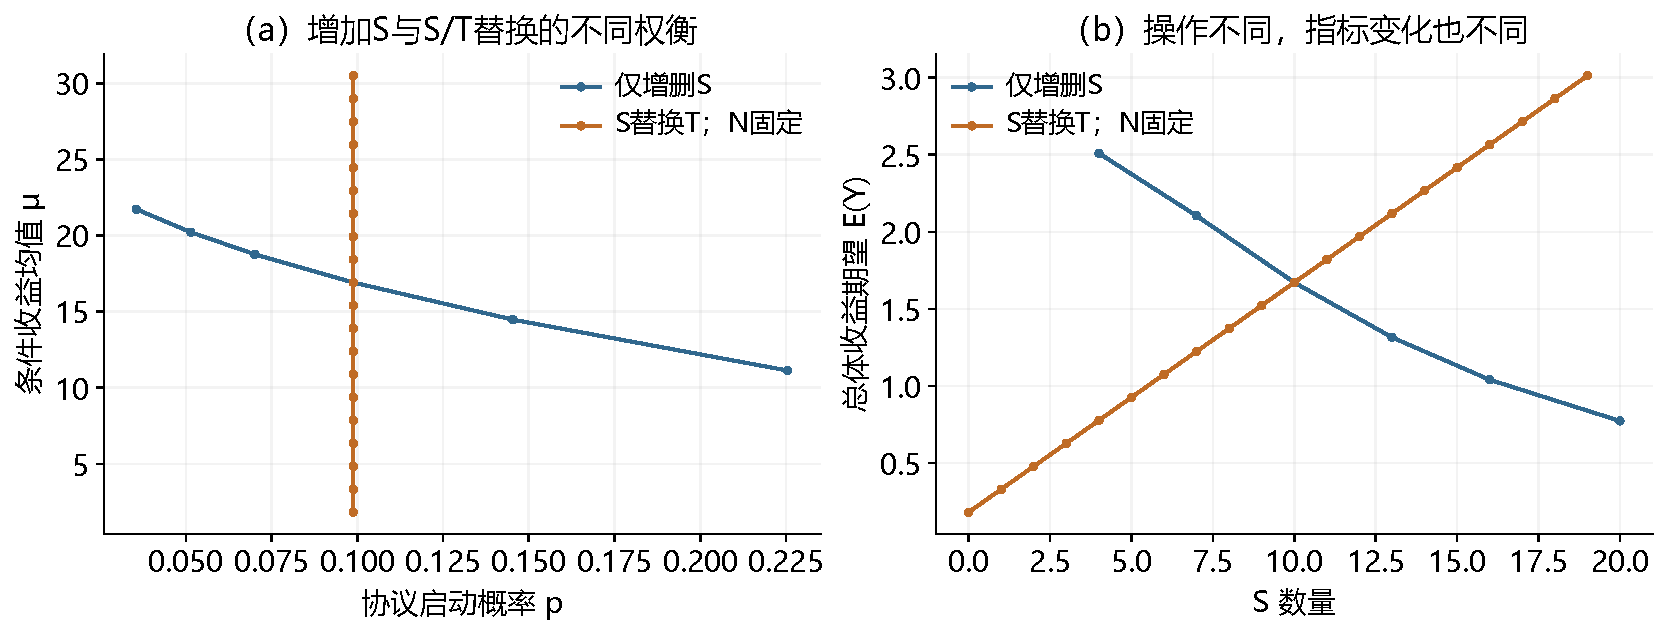
\includegraphics[width=\linewidth]{10_construction_tradeoffs.pdf}
\caption{增加S与固定规模S/T替换的不同效果，曲线均为精确理论值。
左图比较启动概率与条件均值，右图比较总体均值。}\label{fig:tradeoff}
\end{figure}

直接增加6张S后，总体标准差虽从5.5528降至4.7599，
零收益概率却从90.4490\%升至94.9149\%，$\CV(Y)$从3.3223升至4.5763。
总体标准差下降的同时，零收益更加频繁，故应结合均值、零收益率与变异系数解读。
固定$N$做S/T替换时，成功概率恒定，条件与总体格挡均值同向上升。
攻击牌T的输出价值可以在进一步的攻防联合模型中考察。

复制关键牌则同时改变可及性与剩余非攻击比例。
以C替换T或S具有相同的启动概率，却有不同的条件均值，
因为两种来源使非攻击牌总数的变化不同。
因此，相同总牌数下，不同类别的构成依然产生不同的收益分布；
构筑比较应具体说明增删或替换的牌类与数量。

\section{蒙特卡洛模拟与统计验证}\label{sec:simulation}
\subsection{独立排列、估计量与区间}
理论计算采用精确组合数与有理数；模拟则独立生成带编号实体牌的随机排列，
从前$n$张判断$I$，并读取随后$h$张计算$X$、$Y$。
107组不同的“牌组、$n$、$h$”配置各运行$m=200\,000$次，
基准另做$1\,000\,000$次独立复验。
伪随机生成器为NumPy的PCG64，根种子为20261114，
不同配置、复验和收敛实验按独立派生流执行。
同一排列上的多个前缀统计量具有相关性。

设第$r$次试验结果为$(I_r,Y_r)$，成功数
$K=\sum_{r=1}^m I_r$。使用
\begin{equation}\label{eq:estimators}
\widehat p=\frac Km,\qquad
\overline Y=\frac1m\sum_{r=1}^mY_r,\qquad
\widehat\mu=\frac1K\sum_{r:I_r=1}Y_r
\end{equation}
估计启动概率、总体均值与条件均值。
条件指标以成功次数$K$作为样本量。
所有配置的联合分布均核对$\sum_xJ_x=p$；
条件与总体PMF分别核对归一性，并检验式\eqref{eq:total-moments}。
当$p=0$时，总体收益为0，条件指标按未定义处理。

启动比例采用Wilson区间\cite{wilson}。
令$z_{0.975}\approx1.96$为标准正态分位数，则区间为
\begin{equation}\label{eq:wilson}
\frac{\widehat p+z_{0.975}^2/(2m)
\ \pm\ z_{0.975}
\sqrt{\widehat p(1-\widehat p)/m+z_{0.975}^2/(4m^2)}}
{1+z_{0.975}^2/m}.
\end{equation}
总体均值采用$\overline Y\pm z_{0.975}s_Y/\sqrt m$，
其中$s_Y^2$是分母为$m-1$的无偏样本方差；
条件均值区间相应使用成功样本标准差与$\sqrt K$。
有界收益保证有限方差，大数定律给出估计收敛，
中心极限定理给出这些均值区间的渐近依据\cite{blitzstein}。

\subsection{基准验证与抽样误差}
表\ref{tab:validation}保留两次独立运行。
20万次主实验中，启动率与总体均值的95\%区间未覆盖理论值，
对应标准化误差约为$-3.008$与$-3.279$；
条件均值区间覆盖理论值。
100万次独立复验的三个区间均覆盖理论值。
复验使用另一条独立随机流。

\begin{table}[htbp]
\centering\small
\caption{基准精确理论与独立排列模拟；概率用Wilson区间，均值用CLT区间}\label{tab:validation}
\setlength{\tabcolsep}{6pt}
\begin{tabular}{lrrrrr}
\toprule
指标 & 排列次数 & 条件样本量$K$ & 精确理论 & 模拟估计 & 95\%置信区间 \\
\midrule
$p$ & 200,000 & --- & 0.098814 & 0.096825 & [0.095537, 0.098129] \\
$p$ & 1,000,000 & --- & 0.098814 & 0.098648 & [0.098065, 0.099234] \\
$\mu$ & 200,000 & 19,365 & 16.914286 & 16.846476 & [16.742636, 16.950316] \\
$\mu$ & 1,000,000 & 98,648 & 16.914286 & 16.880464 & [16.834366, 16.926562] \\
$\mathbb E(Y)$ & 200,000 & --- & 1.671372 & 1.631160 & [1.607123, 1.655197] \\
$\mathbb E(Y)$ & 1,000,000 & --- & 1.671372 & 1.665224 & [1.654361, 1.676087] \\
\bottomrule
\end{tabular}

\end{table}

95\%置信区间具有重复抽样意义，基准主实验的偏差展示了单次区间的随机性。
在101个非退化配置中，启动率与总体均值的标准化误差绝对值超过1.96的配置
分别为5组与4组。精确计数、全排列核查与随机模拟共同检验了数值实现。

为考察样本量对精度的影响，分别在
$m=2\,000,10\,000,50\,000,200\,000$下独立重复30次，
计算估计误差的均方根（RMSE）。
启动率与总体均值的理论标准误为
\begin{equation}\label{eq:mc-scale}
\operatorname{SE}(\widehat p)=\sqrt{\frac{p(1-p)}m},\qquad
\operatorname{SE}(\overline Y)=\sqrt{\frac{\V(Y)}m}.
\end{equation}
图\ref{fig:convergence}中，实测RMSE与理论尺度相符：
总体均值RMSE由0.117652降至0.012047，理论标准误由0.124165降至0.012416。
样本量扩大5倍时，理论标准误缩小为原来的$1/\sqrt5$；
重复实验的RMSE围绕相应尺度变化。

\begin{figure}[htbp]
\centering
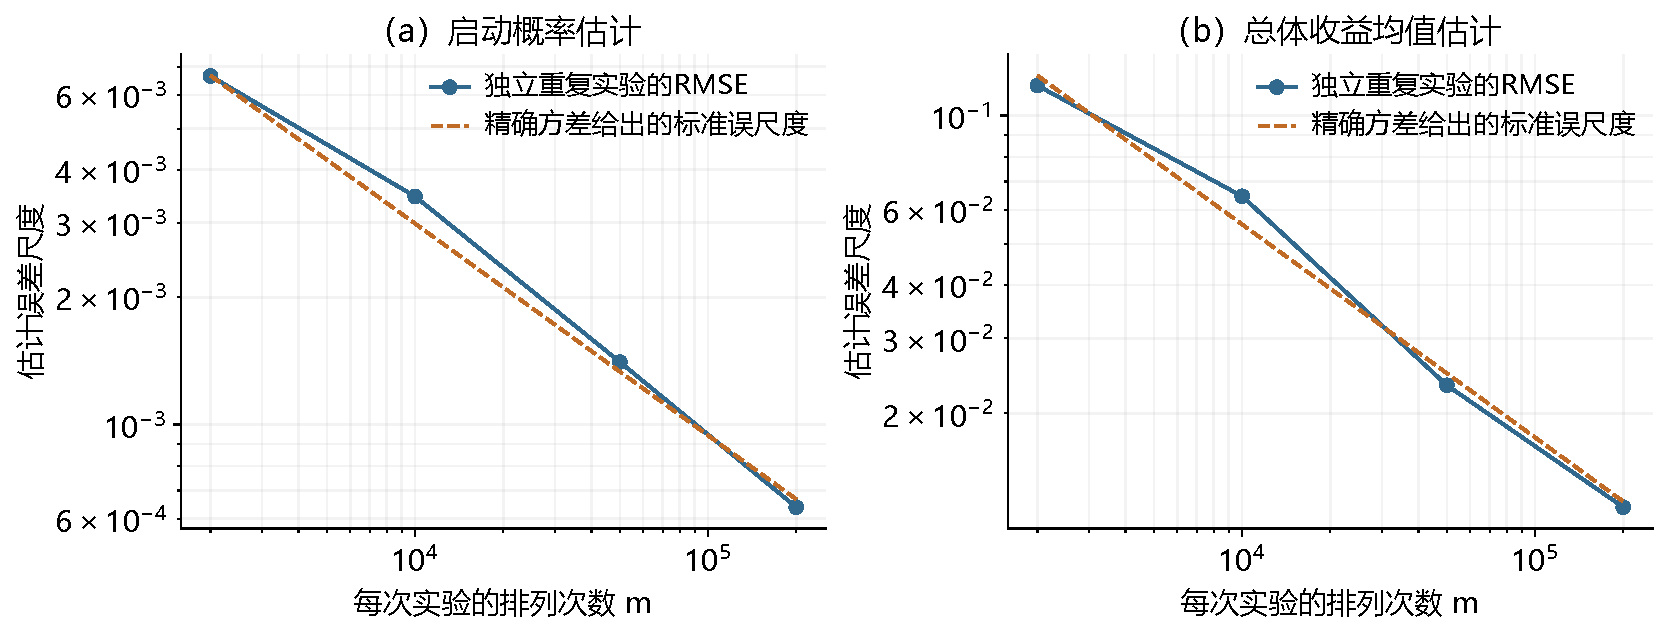
\includegraphics[width=\linewidth]{09_convergence.pdf}
\caption{不同样本量下各30次独立重复的RMSE与精确方差给出的标准误尺度；
双对数坐标中的理论斜率为$-1/2$。}\label{fig:convergence}
\end{figure}

\FloatBarrier
\section{结论与展望}
本文用联合可及性与条件回报两个层次，刻画了有限随机卡组的协同收益。
容斥与尾和公式给出组件见齐概率和首次见齐时间；
有限前缀的顺序计数进一步表明，组件齐全与满足特定先后要求是不同事件。
同洗牌的条件超几何混合保留了前后阶段的组成依赖，
使条件收益与总体收益可以在统一样本空间中计算。

固定牌组规模时，交换性把条件收益均值与方差分别化为一次式与二次式，
并确定条件方差在普通非攻击牌数为9时最大。
全方差分解揭示，基准总体波动主要来自成功与失败两类条件均值的差异。
明确区分增删与替换后，增加普通非攻击牌所产生的条件回报提升，
可以与组件可及性下降同时发生；总体期望由两者共同决定。
这些结果说明，稳定性需要结合事件概率、条件分布与操作成本解释。

后续研究可以引入抽牌反馈、重新洗牌、能量约束和出牌策略，
建立动态状态转移模型，考察卡组构筑对启动效率与消耗收益的影响。

\label{maintext:end}
\FloatBarrier
\clearpage
\bibliographystyle{unsrtnat}
{\small\raggedright
\bibliography{references}
\par}
\appendix
\section*{附录：数据来源与复现}
\addcontentsline{toc}{section}{附录：数据来源与复现}
\noindent\textbf{数据来源与复现。}
文中数值与图表来自本文定义的抽象随机实验，
由精确组合计算和Python实体排列模拟生成。
107组主实验、基准复验及精度实验共使用$30\,260\,000$次排列。
复现环境为Python 3.13.11、NumPy 2.5.4、Matplotlib 3.11.2。
项目保存配置、整数直方图、理论分数、种子和源文件摘要；
正文表格由这些既有结果自动提取，7组矢量图沿用已核验数据与绘图程序，
并为A4印刷放大标注字号；原始图另行保留。
论文目录中的复现说明列出了完整命令及数据对应关系。

\medskip
\noindent\textbf{推广计数。}
对多副本A/B/C构筑，若设置阶段相应计数为$i,j,\ell$，
S计数为$u$，则成功要求$i,j,\ell\ge1$，剩余可消耗数为
\[
M=(a-i)+(b-j)+(c-\ell)+(s-u).
\]
设置计数的组合权重为
\[
q(i,j,\ell,u)=
\frac{\binom ai\binom bj\binom c\ell\binom su
\binom{d+t}{n-i-j-\ell-u}}{\binom Nn}.
\]
给定计数后，收益分布为$\operatorname{Hypergeom}(N-n,M,h)$；
按权重混合即推广式\eqref{eq:joint}，并保留单对A/B激活的固定收益系数8。

\end{document}
